\documentclass[letterpaper,10pt]{article}
\title{Assignment 2 Report - Logistic Regression with \(L_2\) Regularization}
\author{Helena Bales and Natalie Suderman\\ \\ CS343 - Spring 2017}
\usepackage[pdftex]{graphicx}
\usepackage{tikz}
\usepackage{float}

\parindent = 0.0 in
\parskip = 0.1 in

\begin{document}
\maketitle

\tableofcontents
\clearpage

\section{Introduction}
This report covers the second implementation assignment for Machine Learning and Data Mining. This 
assignment covers logistic regression with \(L_2\) Regularization using data from USPS's database of 
handwritten digits. This program will distinguish handwritten number 4's from 9's. Each digit is an 
image of size 16x16 pixels. The dataset that we will use was given on the class website and contains 
700 training samples and 400 testing samples. We used the batch decent gradient algorithm to train 
to train the classifier. In order to complete this, we had to pick a reasonable learning rate and 
identify a reasonable stopping condition. These dicisions will be covered in the Question 1 section 
below. Following completion of question 1, we reran the model from the beginning and plotted each 
decent gradient iteration. These plots, as well as an interpretation of the plots, can be found in 
the Question 2 section below. The next question involves \(L_2\) regularization. We will modify the 
code to find the gradient for the objective function \(L(w)\) given in the assignment and modify the 
batch gradient descent algorithm with this new gradient. The process and pseudocode for the \(L_2\) 
regularization will be covered in the Question 3 section below. Finally, the Question 4 section will 
cover the implementation of the change discussed in the Question 3 section. This implementation will 
then be evaluated based on their accuracies of the training and testing achieved using different 
\(\lambda\) values.

\section{Question 1}
\subsection{Problem Statement}
Implement the batch gradient descent algorithm to train a binary logistic regression classifier. 
The behavior of Gradient descent can be strongly in influenced by the learning rate. Experiment with 
different learning rates, report your observation on the convergence behavior of the gradient 
descent algorithm. For your implementation, you will need to decide a stopping condition. You might 
use a fixed number of iterations, the change of the objective value (when it ceases to be 
significant) or the norm of the gradient (when it is smaller than a small threshold). Note, if you 
observe an overflow, then your learning rate is too big, so you need to try smaller learning rates.

\subsection{Convergence Behavior}
     \begin{figure}[ht]
    \centering
   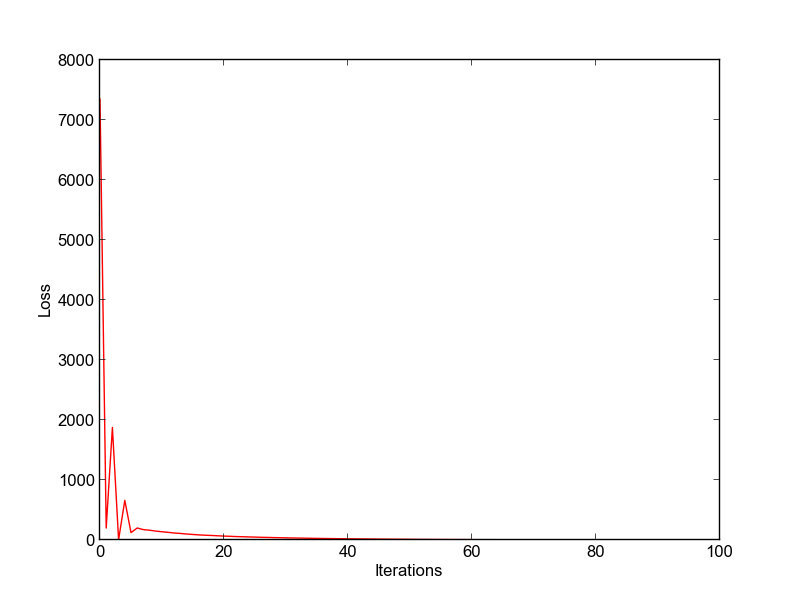
\includegraphics[width=250pt]{convergenceClose.png}
    \caption{Convergence of loss function}
    \label{fig:Convergence of loss function over iterations}
    \end{figure}
As the data was run multiple times the loss function was minimized.
We ran about 1000 iterations, but in order to focus on the interesting parts, only the first 100 iterations were included in the interest of space.   

\subsection{Learning Rate}
The learning rate we decided on was .00000001. 
Learning rates bigger than .000001 always gave us an overflow error before the gradient converged.
\subsection{Stopping Condition}
Originally, we used the stopping condition ||dNew-dOld||2 < .01, but the way that I calculated accuracy didn't provide enough significant digits for this to be successful.
Instead we chose to stop using a set number of iterations. In our case, about 1000 iterations was sufficient to see the convergence.  

\section{Question 2}
\subsection{Problem Statement}
Once you identify a suitable learning rate, rerun the training of the model from the beginning. For 
each gradient descent iteration, plot the training accuracy and the testing accuracy of your model 
as a function of the number of gradient descent iterations. What trend do you observe?

\subsection{Plots}
     \begin{figure}[ht]
    \centering
   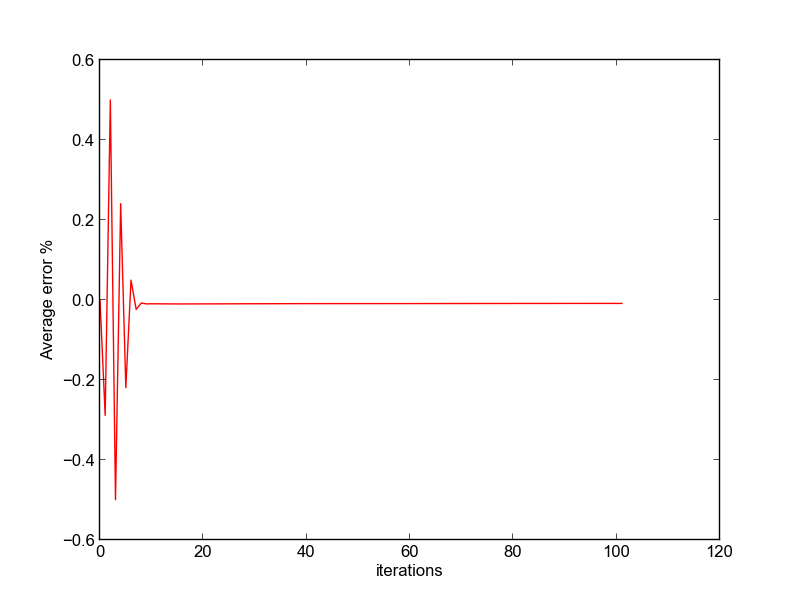
\includegraphics[width=250pt]{gradientDescentImprovement.png}
    \caption{Plot of accuracy of each data set}
    \label{fig:Plot of accuracy over iterations. Red is training data}
    \end{figure}
\subsection{Interpretation of Data}
The test data immediately begins at a higher accuracy, because it has the advantage of starting with the weight vector calculated from the train data. You can see that after several iterations the model improves dramatically, and rests at about a 95\% accuracy for both sets of data.


\section{Question 3}
\subsection{Problem Statement}
As discussed in class, Logistic regression is typically used with regularization. We will explore 
\(L_2\) regularization for this question. In particular, we will the following objective with an 
additional regularization term that is equal to the squared Euclidean norm of the weight vector.

Where the loss function l is the same as introduced in class (slide 7 of the logistic regression 
notes). Find the gradient for this objective function and modify the batch gradient descent \
algorithm with this new gradient. Provide the pseudo code for your modified algorithm.

\subsection{Method}
I will be finding the gradient of the following objective function:
\[L(w) = \sum_{i=1}^n l(g(w^T x^i), y^i) + \frac{1}{2} \lambda ||w||_2^2  \]
Where \(l(g(w^T x^i), y^i) = \{^{-log(g(w^T x^i)), if y^i = 1}_{-log(1-g(w^T x^i)), if y^i = 0} \)

\subsection{Calculating Gradient}
\[ l(g(w^T x^i), y^i) = -y^i log(P(y=1 | x^i; w)) - (1-y^i) log(1-P(y=1 | x^i; w)) \]
\[ l(g(w^T x^i), y^i) = -y^i log(g(w^T x^i)) - (1-y^i) log(1 - g(w^T x^i)) \]
\[ \bigtriangledown g(w^T x^i) = g(w^T x^i) (1 - g(w^T x^i)) x^i \]
\[ \bigtriangledown l(g(w^T x^i), y^i) = -(y^i - g(w^T x^i)) x^i \]

\subsection{Pseudocode}
\begin{enumerate}
	\item{Start with an initial guess \(w^0\).}
	\item{Find the direction of steepest descent \(= - \bigtriangledown f(w) \)}
	\item{Take a step towards that direction \( = w^{t+1} = w^T - \bigtriangledown f(w^T) \)}
	\item{Repeat until no local improvement is possible.}
\end{enumerate}

\section{Question 4}
\subsection{Problem Statement}

\subsection{Implementation of Pseudocode from Question 3}
\subsection{Evaluation of Implementation}

\section{Conclusion}

\end{document}
